%! suppress = MissingImport
If you have not already done so, download \textit{CowPi.zip}.

\begin{description}
    \checkoffitem{In the Arduino IDE's Sketch menu, install the CowPi library: \\
        \textit{Sketch} $\rightarrow$ \textit{Include Library} $\rightarrow$ \textit{Add .ZIP Library\dots}
        (see Figure~\ref{fig:add-library}).}
        \begin{itemize}
            \item In the resulting popup window, navigate to your ``Downloads'' directory (or wherever you saved \textit{CowPi.zip} after downloading it), click on \textit{CowPi.zip}, and click on ``Open''.
            \item If you have an earlier version of the CowPi library installed, you will be prompted to confirm that you wish to replace the earlier version (Figure~\ref{fig:update-library});
                click on ``Yes''.
            \item You should immediately get the message, ``Library Installed''.
        \end{itemize}
    \checkoffitem{Close the Arduino IDE and then re-open the Arduino IDE\@.}
\end{description}

\begin{figure}
    \centering
    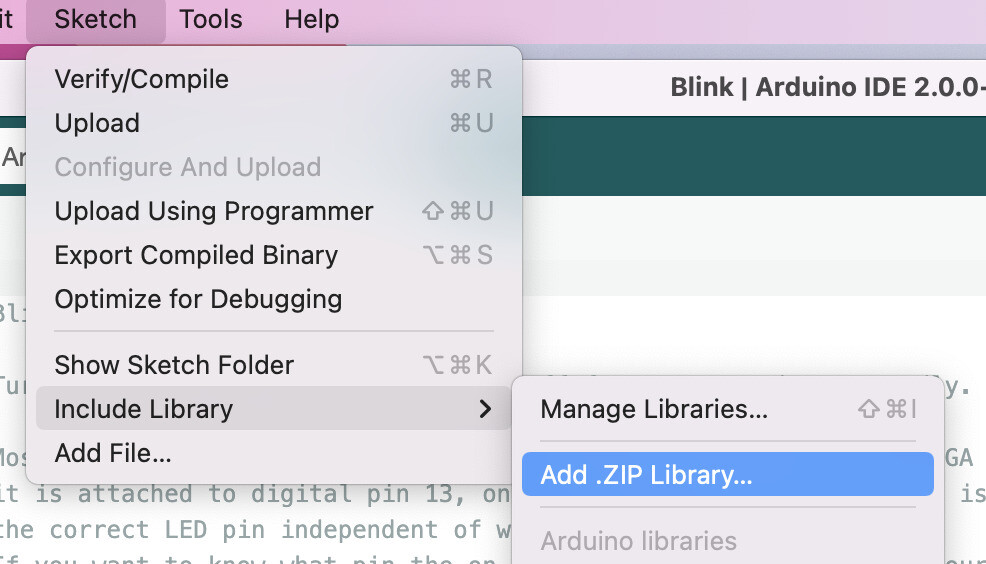
\includegraphics[width=0.5\textwidth]{direct/library/add-zip-library}
    \caption{Adding a downloaded library to Arduino IDE. \label{fig:add-library}}
\end{figure}

\begin{figure}
    \centering
    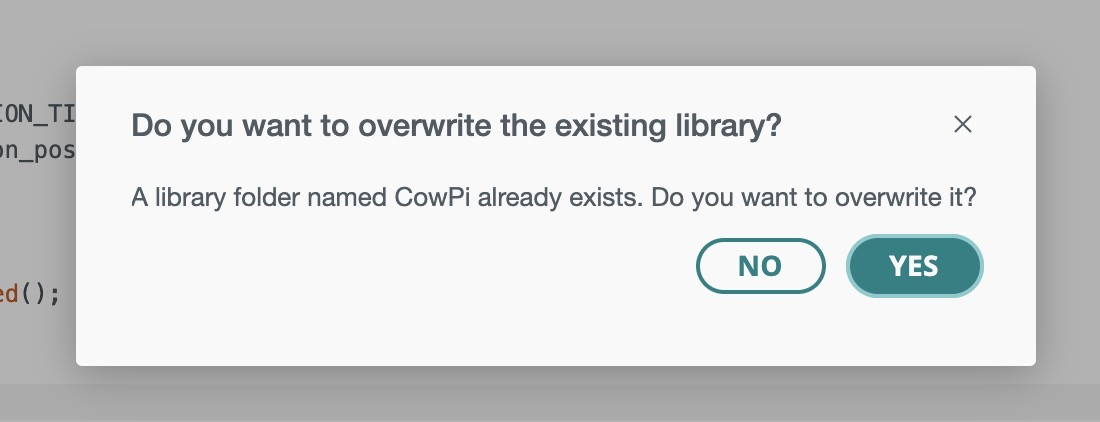
\includegraphics[width=0.5\textwidth]{direct/library/update-zip-library}
    \caption{Replacing a downloaded library in the Arduino IDE. \label{fig:update-library}}
\end{figure}

From the Arduino IDE's File menu, you now have additional examples under the ``Examples from Custom Libraries'' heading: \\
\textit{File} $\rightarrow$ \textit{Examples} $\rightarrow$ \textit{CowPi}
(see Figure~\ref{fig:library-examples}).

\begin{figure}
    \centering
    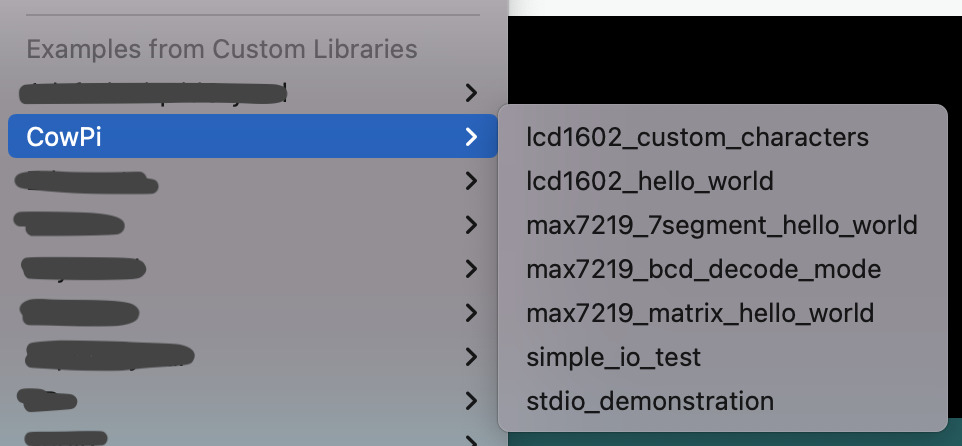
\includegraphics[width=0.5\textwidth]{direct/library/library-examples}
    \caption{Code examples for the class hardware kit are now available. \label{fig:library-examples}}
\end{figure}

\begin{description}
    \checkoffitem{Open \textit{simple\_io\_test}.}
    \checkoffitem{Find these lines in the \function{setup()} function:}
\begin{lstlisting}[numbers=left, firstnumber=13]
    cowpi_setup(SPI);
//    cowpi_setup(I2C);
\end{lstlisting}
\end{description}

%! suppress = NonMatchingIf
\ifdefstring{\serialprotocol}{SPI}{
    \begin{description}
        \checkoffitem{Make sure that the \lstinline{cowpi_setup(SPI)} line is uncommented and that the \lstinline{cowpi_setup(I2C)} line is commented-out.}
        \checkoffitem{The hardware kit is configured slightly differently, depending on which serial communication protocol is used with the display module, and this semester we will use the SPI protocol.}
    \end{description}
}{}
%! suppress = NonMatchingIf
\ifdefstring{\serialprotocol}{I2C}{
    \begin{description}
        \checkoffitem{Comment-out the \lstinline{cowpi_setup(SPI)} line, and uncomment the \lstinline{cowpi_setup(I2C)} line.}
        \checkoffitem{The hardware kit is configured slightly differently depending on which serial communication protocol is used with the display module, and this semester we will use the I$^2$C protocol.}
    \end{description}
}{}

\begin{description}
    \checkoffitem{Compile and upload \textit{simple\_io\_test.ino} to your \developmentboard\ in the same manner that you did for \textit{Blink.ino}.}
    \checkoffitem{Open the Arduino IDE's Serial Monitor: Tools $\rightarrow$ Serial Monitor.}
\end{description}
You will see the message:

\begin{verbatim}
    CowPi library version 0.4.0
    This demonstration makes no assumptions about your CowPi's display module,
        so your display module may display garbage -- that's okay.
    The `cowpi_setup` function will be called with either `SPI` or `I2C` so that
        the CowPi library knows where your slider switches are.
        Your instructor should have told you which to use.
    The simple I/O test will print the status of the keypad and of each
        button, switch, and LED every half-second.
    Press the Enter key on your host computer's keyboard to start.
\end{verbatim}

While the Enter key would be appropriate on a ``raw'' serial terminal, for the Arduino IDE's Serial Monitor, you will start the rest of the program using one of three techniques:
\begin{description}
    \item[If you are running Arduino IDE 1.8] then place the cursor in the Serial Monitor's text-entry field and click on the ``Send'' button.
    \item[If you are running Arduino IDE 2.0 on Windows or Linux] then place the cursor in the Serial Monitor's text-entry field and press Control-Enter.
    \item[If you are running Arduino IDE 2.0 on MacOS] then place the cursor in the Serial Monitor's text-entry field and press Command-Enter.
\end{description}

After you start the rest of the program, the \developmentboard\ will send a message to the Serial Monitor every half-second:

\begin{verbatim}
    Keypad:               Column pins:  1111    Keypad NAND: 0
    Left switch: RIGHT    Right switch: RIGHT
    Left button: UP       Right button: UP      Button NAND: 0
    Left LED:    OFF      Right LED:    OFF
\end{verbatim}

For now, no other output is possible.
